%% abtex2-modelo-relatorio-tecnico.tex, v-1.9.5 laurocesar
%% Copyright 2012-2015 by abnTeX2 group at http://www.abntex.net.br/ 
%%
%% This work may be distributed and/or modified under the
%% conditions of the LaTeX Project Public License, either version 1.3
%% of this license or (at your option) any later version.
%% The latest version of this license is in
%%   http://www.latex-project.org/lppl.txt
%% and version 1.3 or later is part of all distributions of LaTeX
%% version 2005/12/01 or later.
%%
%% This work has the LPPL maintenance status `maintained'.
%% 
%% The Current Maintainer of this work is the abnTeX2 team, led
%% by Lauro César Araujo. Further information are available on 
%% http://www.abntex.net.br/
%%
%% This work consists of the files abntex2-modelo-relatorio-tecnico.tex,
%% abntex2-modelo-include-comandos and abntex2-modelo-references.bib
%%

% ------------------------------------------------------------------------
% ------------------------------------------------------------------------
% abnTeX2: Modelo de Relatório Técnico/Acadêmico em conformidade com 
% ABNT NBR 10719:2011 Informação e documentação - Relatório técnico e/ou
% científico - Apresentação
% ------------------------------------------------------------------------ 
% ------------------------------------------------------------------------

\documentclass[
	% -- opções da classe memoir --
	12pt,				% tamanho da fonte
	openright,			% capítulos começam em pág ímpar (insere página vazia caso preciso)
	oneside,			% para impressão em verso e anverso. Oposto a oneside
	a4paper,			% tamanho do papel. 
	% -- opções da classe abntex2 --
	%chapter=TITLE,		% títulos de capítulos convertidos em letras maiúsculas
	%section=TITLE,		% títulos de seções convertidos em letras maiúsculas
	%subsection=TITLE,	% títulos de subseções convertidos em letras maiúsculas
	%subsubsection=TITLE,% títulos de subsubseções convertidos em letras maiúsculas
	% -- opções do pacote babel --
	english,			% idioma adicional para hifenização
	french,				% idioma adicional para hifenização
	spanish,			% idioma adicional para hifenização
	brazil,				% o último idioma é o principal do documento
	]{abntex2}


% ---
% PACOTES
% ---

% ---
% Pacotes fundamentais 
% ---
\usepackage{lmodern}			% Usa a fonte Latin Modern
\usepackage[T1]{fontenc}		% Selecao de codigos de fonte.
\usepackage[utf8]{inputenc}		% Codificacao do documento (conversão automática dos acentos)
\usepackage{indentfirst}		% Indenta o primeiro parágrafo de cada seção.
\usepackage{color}				% Controle das cores
\usepackage{graphicx}			% Inclusão de gráficos
\usepackage{microtype} 			% para melhorias de justificação
% ---

% ---
% Pacotes adicionais, usados no anexo do modelo de folha de identificação
% ---
\usepackage{multicol}
\usepackage{multirow}
% ---
	
% ---
% Pacotes adicionais, usados apenas no âmbito do Modelo Canônico do abnteX2
% ---
\usepackage{lipsum}				% para geração de dummy text
% ---
\usepackage{amsmath}
\usepackage[locale=FR]{siunitx}
% ---
% Pacotes de citações
% ---
\usepackage[brazilian,hyperpageref]{backref}	 % Paginas com as citações na bibl
\usepackage[num,overcite]{abntex2cite}	% Citações padrão ABNT
\citebrackets[]

% --- 
% CONFIGURAÇÕES DE PACOTES
% --- 

% ---
% Configurações do pacote backref
% Usado sem a opção hyperpageref de backref
\renewcommand{\backrefpagesname}{Citado na(s) página(s):~}
% Texto padrão antes do número das páginas
\renewcommand{\backref}{}
% Define os textos da citação
\renewcommand*{\backrefalt}[4]{
	\ifcase #1 %
		Nenhuma citação no texto.%
	\or
		Citado na página #2.%
	\else
		Citado #1 vezes nas páginas #2.%
	\fi}%
% ---

% ---
% Informações de dados para CAPA e FOLHA DE ROSTO
% ---
\titulo{Relatório 1\\Laboratório de Eletrônica - ENG10045}
\autor{Cassiano Translatti Furlani\\Oberdan Costa dos Santos}
\local{Porto Alegre - RS}
\data{2018}
\instituicao{
  Universidade Federal do Rio Grande do Sul - UFRGS
  \par
  Departamento de Engenharia Elétrica
  \par
  Programa de Graduação
  \par
  Professor: Chrystian Lenon Remes}
% O preambulo deve conter o tipo do trabalho, o objetivo, 
% o nome da instituição e a área de concentração 
\preambulo{	Relatório no qual consta um projeto de uma placa de circuito impresso (PCI), 
simulação nos softwares já visto em outras disciplinas e o dimensionamento térmico de um dissipador.}
% ---

% ---
% Configurações de aparência do PDF final

% alterando o aspecto da cor azul
\definecolor{blue}{RGB}{41,5,195}

% informações do PDF
\makeatletter
\hypersetup{
     	%pagebackref=true,
		pdftitle={\@title}, 
		pdfauthor={\@author},
    	pdfsubject={\imprimirpreambulo},
	    pdfcreator={LaTeX with abnTeX2},
		pdfkeywords={abnt}{latex}{abntex}{abntex2}{relatório técnico}, 
		colorlinks=true,       		% false: boxed links; true: colored links
    	linkcolor=blue,          	% color of internal links
    	citecolor=blue,        		% color of links to bibliography
    	filecolor=magenta,      		% color of file links
		urlcolor=blue,
		bookmarksdepth=4
}
\makeatother
% --- 

% --- 
% Espaçamentos entre linhas e parágrafos 
% --- 

% O tamanho do parágrafo é dado por:
\setlength{\parindent}{1.3cm}

% Controle do espaçamento entre um parágrafo e outro:
\setlength{\parskip}{0.2cm}  % tente também \onelineskip

% ---
% compila o indice
% ---
\makeindex
% ---

% ----
% Início do documento
% ----
\begin{document}

% Seleciona o idioma do documento (conforme pacotes do babel)
%\selectlanguage{english}
\selectlanguage{brazil}

% Retira espaço extra obsoleto entre as frases.
\frenchspacing 

% ----------------------------------------------------------
% ELEMENTOS PRÉ-TEXTUAIS
% ----------------------------------------------------------
% \pretextual

% ---
% Capa
% ---
\imprimircapa
% ---

% ---
% Folha de rosto
% (o * indica que haverá a ficha bibliográfica)
% ---
\imprimirfolhaderosto
% ---

% ---
% inserir o sumario
% ---
\pdfbookmark[0]{\contentsname}{toc}
\tableofcontents*
\cleardoublepage
% ---

% ----------------------------------------------------------
% ELEMENTOS TEXTUAIS
% ----------------------------------------------------------
\textual

% ---
% Conteúdo
% ---
% ----------------------------------------------------------
% Introdução (exemplo de capítulo sem numeração, mas presente no Sumário)
% ----------------------------------------------------------
\chapter*{Introdução}
\addcontentsline{toc}{chapter}{Introdução}

Esse relatório tem como objetivo, a partir de ferramentas de simulação de circuitos, mostrar o comportamento de dois circuitos. Além disso, é feito um projeto de uma placa de circuito impressa (PCI) e o cálculo de dimensionamento térmico de um dissipador para o CI LM7805. 

Na simulação dos circuitos, observamaos um filtro passa baixa, que para freqûencias baixas o ganho é próximo de um, e que depois da frequência de corte, seus ganhos tendem a zero. Veremos também um circuito com dois diodos em paralelo. Para a análise destes circuitos, utilizamos o Micro-cap e o PSIM, ambos softwares de simulação de circuitos e vistos anteriormente em outra disciplina.

Para a criação da PCI foi utilizado o software KiCad, as dimensões do indutor utilizado e o tipo de capacitor, podendo ele ser eletrolítico ou cerâmico, foram determinados por dois números, M e N, dados a cada integrante do grupo. Através da média do primeiro número, M, tinha-se a largura do indutor, e a partir do outro, a profundidade. A soma dos dois valores, M+N, determinava o tipo de capacitor, sendo usado um capacitor eletrolítico se a soma der par e um capacitor cerâmico se ímpar.

Finalmente, temos o cálculo de um possível dissipador térmico pra o CI LM7805, para isso utilizamos o \textit{datasheet} do mesmo e cálculos mostrados em aula. 

% ---
\chapter{Ferramentas de Simulação}\label{cap_simul}
% ---
    Para a tarefa 2 proposta da aula 2, temos que primeiramente analisar analiticamente o circuito da figura a). A partir dele, calculamos o $\tau$, $\tau = R*C $, logo $\tau = 1k5 * 100n = 150us$. Para o cálculo da frquência de corte, usamos o valor de $\tau$ anteriormente obtido na fórmula $f = 1/(2\pi\tau)$ e assim a frequência de corte é $f = 1061.033 Hz$. O ganho K, em regime permanente, é dado por $K = Vo/Vi$ onde $Vi$ é a fonte e $Vo$ é a ddp medida no capacitor. Temos, então $K = 1/(1 + 1.5*10^{-4}s)$.
    
    Simulando o circuito a), para achar a frequência de corte:
\begin{figure}[!htb]
    \begin{minipage}{0.5\textwidth}
    \centering
    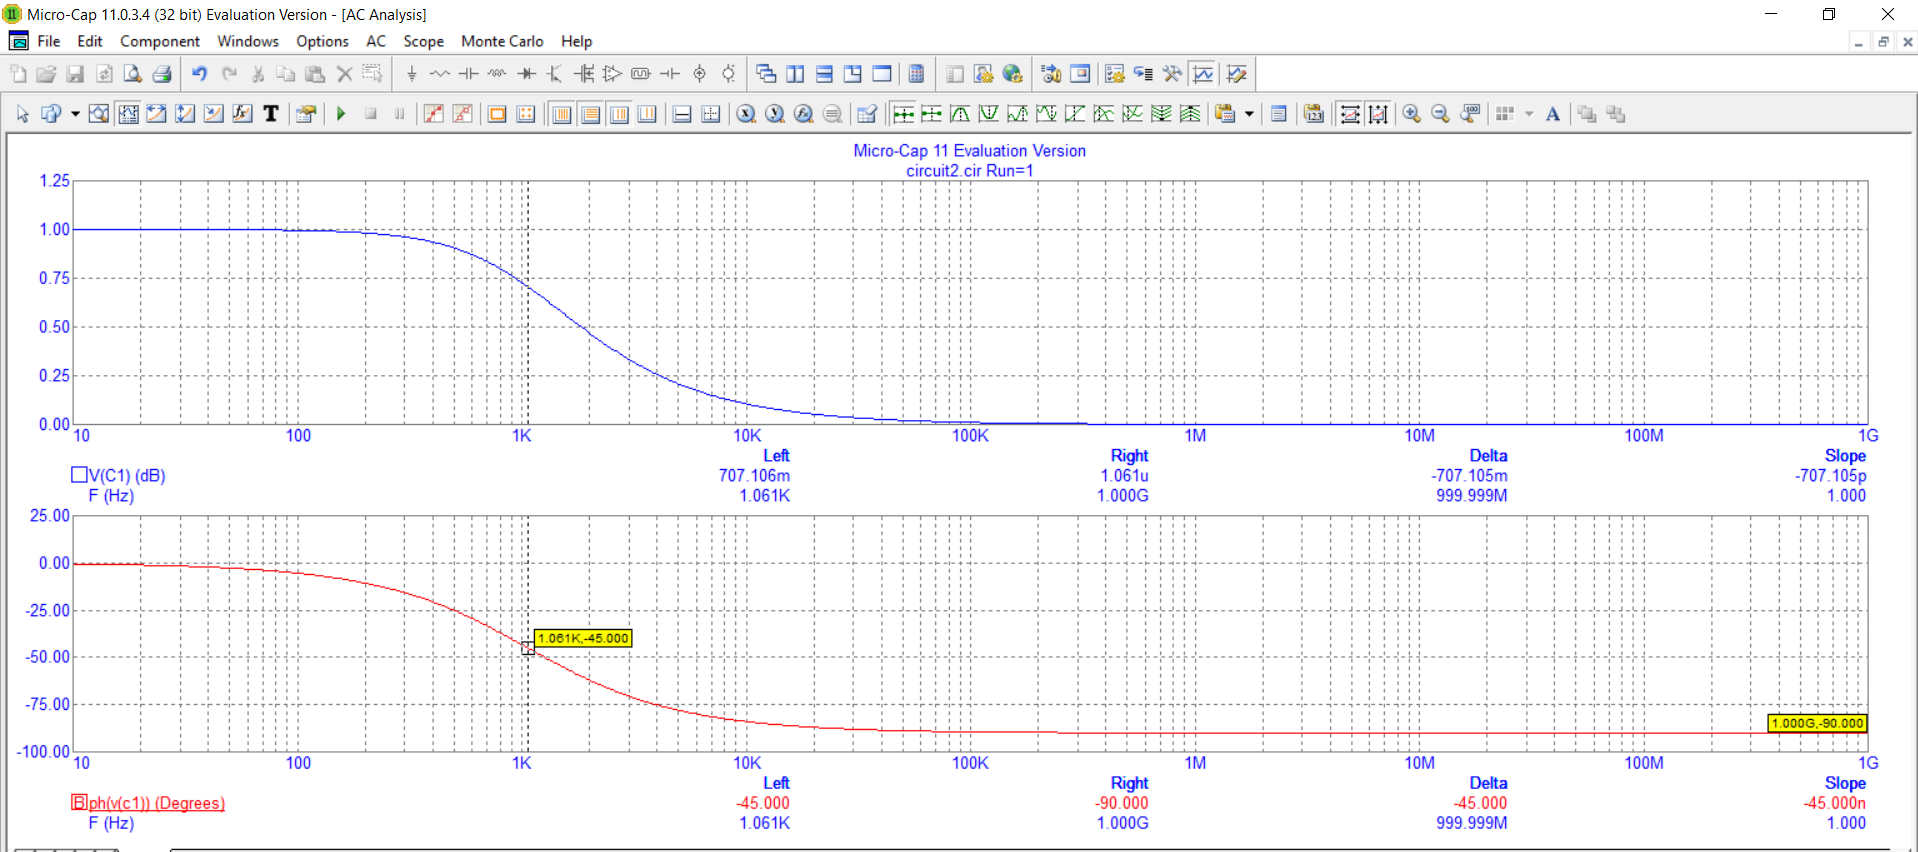
\includegraphics[width = 0.9\textwidth]{Relatorio1_microcap_Bode.png}
    \caption{Simulação no Micro-cap\cite{microcap}}
    \end{minipage}\hfill
    \begin{minipage}{0.5\textwidth}
    \centering
    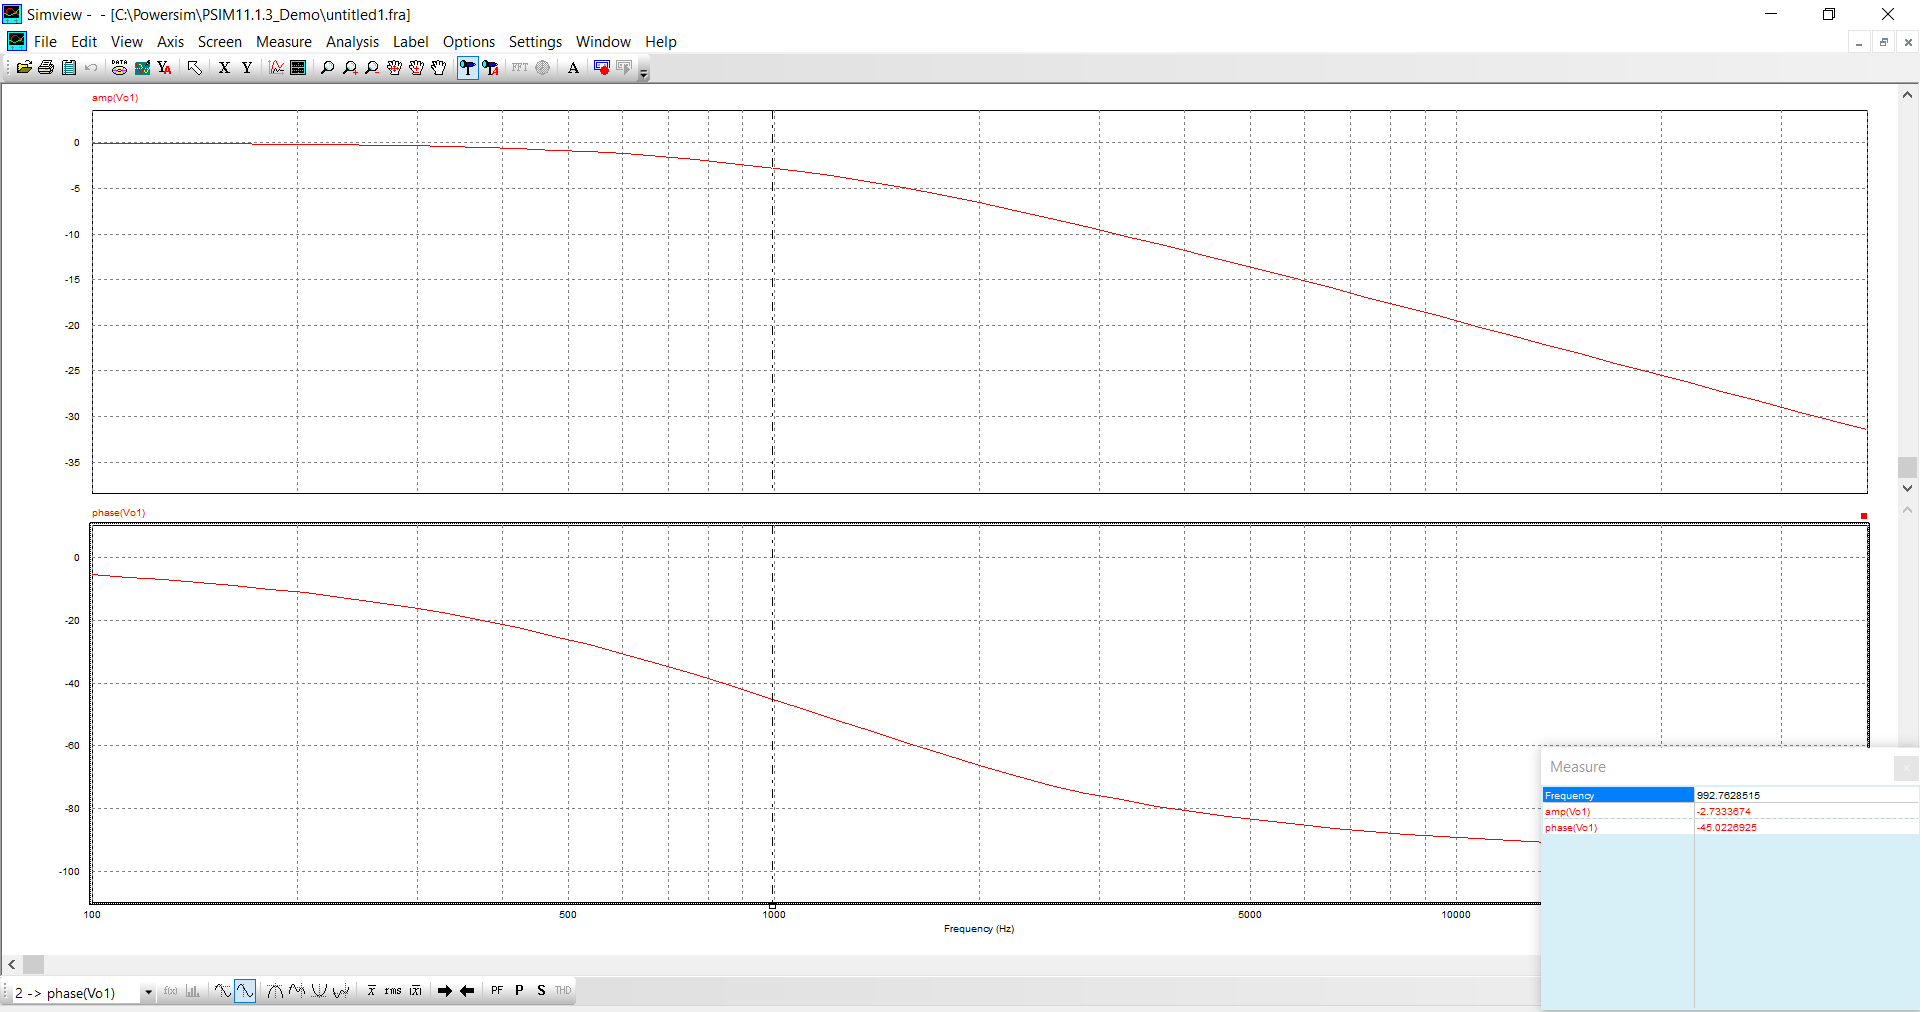
\includegraphics[width = 0.9\textwidth]{Relatorio1_PSIM_Bode.png}
    \caption{Simulação no PSIM\cite{psim}}
    \end{minipage}\hfill
\end{figure}

    Para o resultado do PSIM, mudamos a formade onda para uma senoidal, apenas para o cálcuo da frquência. Com isso, a partir da fase da onda, aos -45graus achamos a frequência de corte em cada simulador. No Micro-cap ficando com 1061Hz e no Psim 992Hz. 
    
    Para encontrar $\tau$, temos:
    
    \begin{figure}[!htb]
    \begin{minipage}{0.5\textwidth}
    \centering
    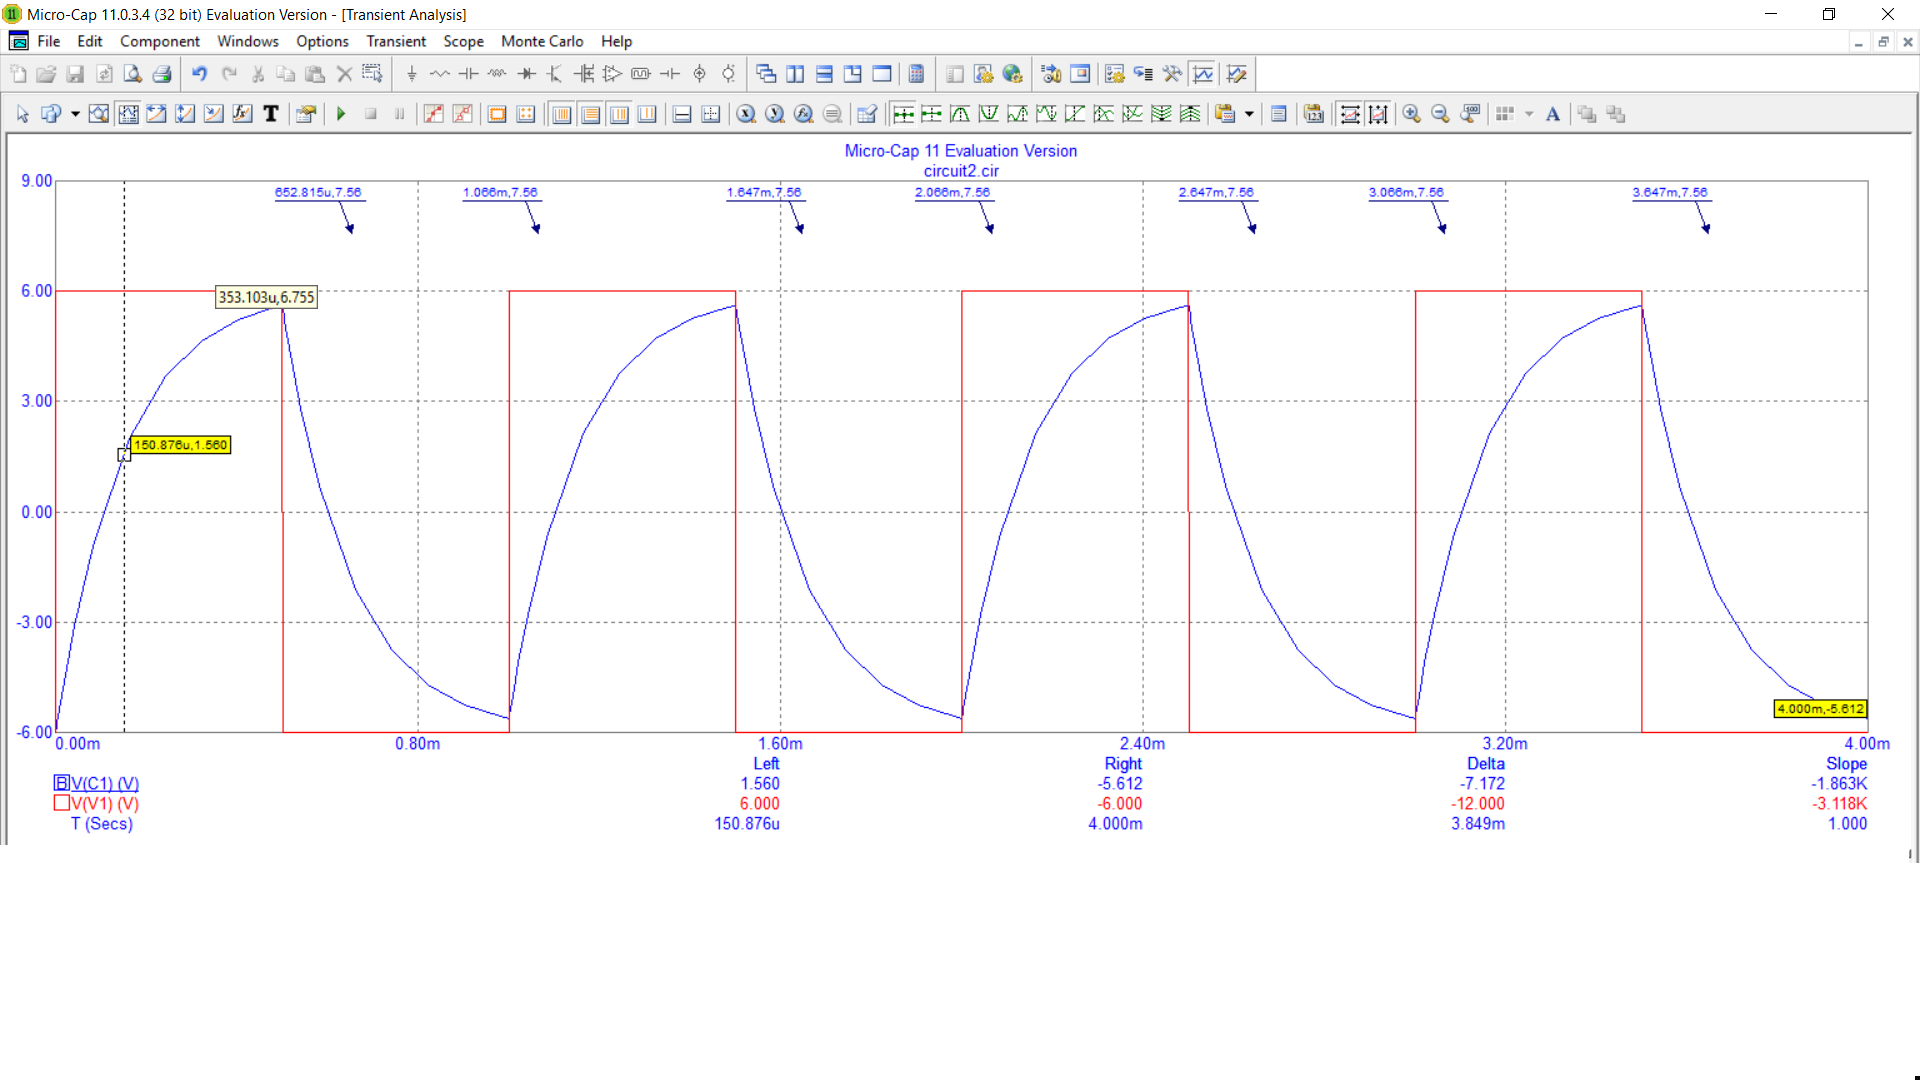
\includegraphics[width = 0.9\textwidth]{Relatorio1_microcap_Tau.png}
    \caption{Simulação no Micro-cap\cite{microcap}}
    \end{minipage}\hfill
    \begin{minipage}{0.5\textwidth}
    \centering
    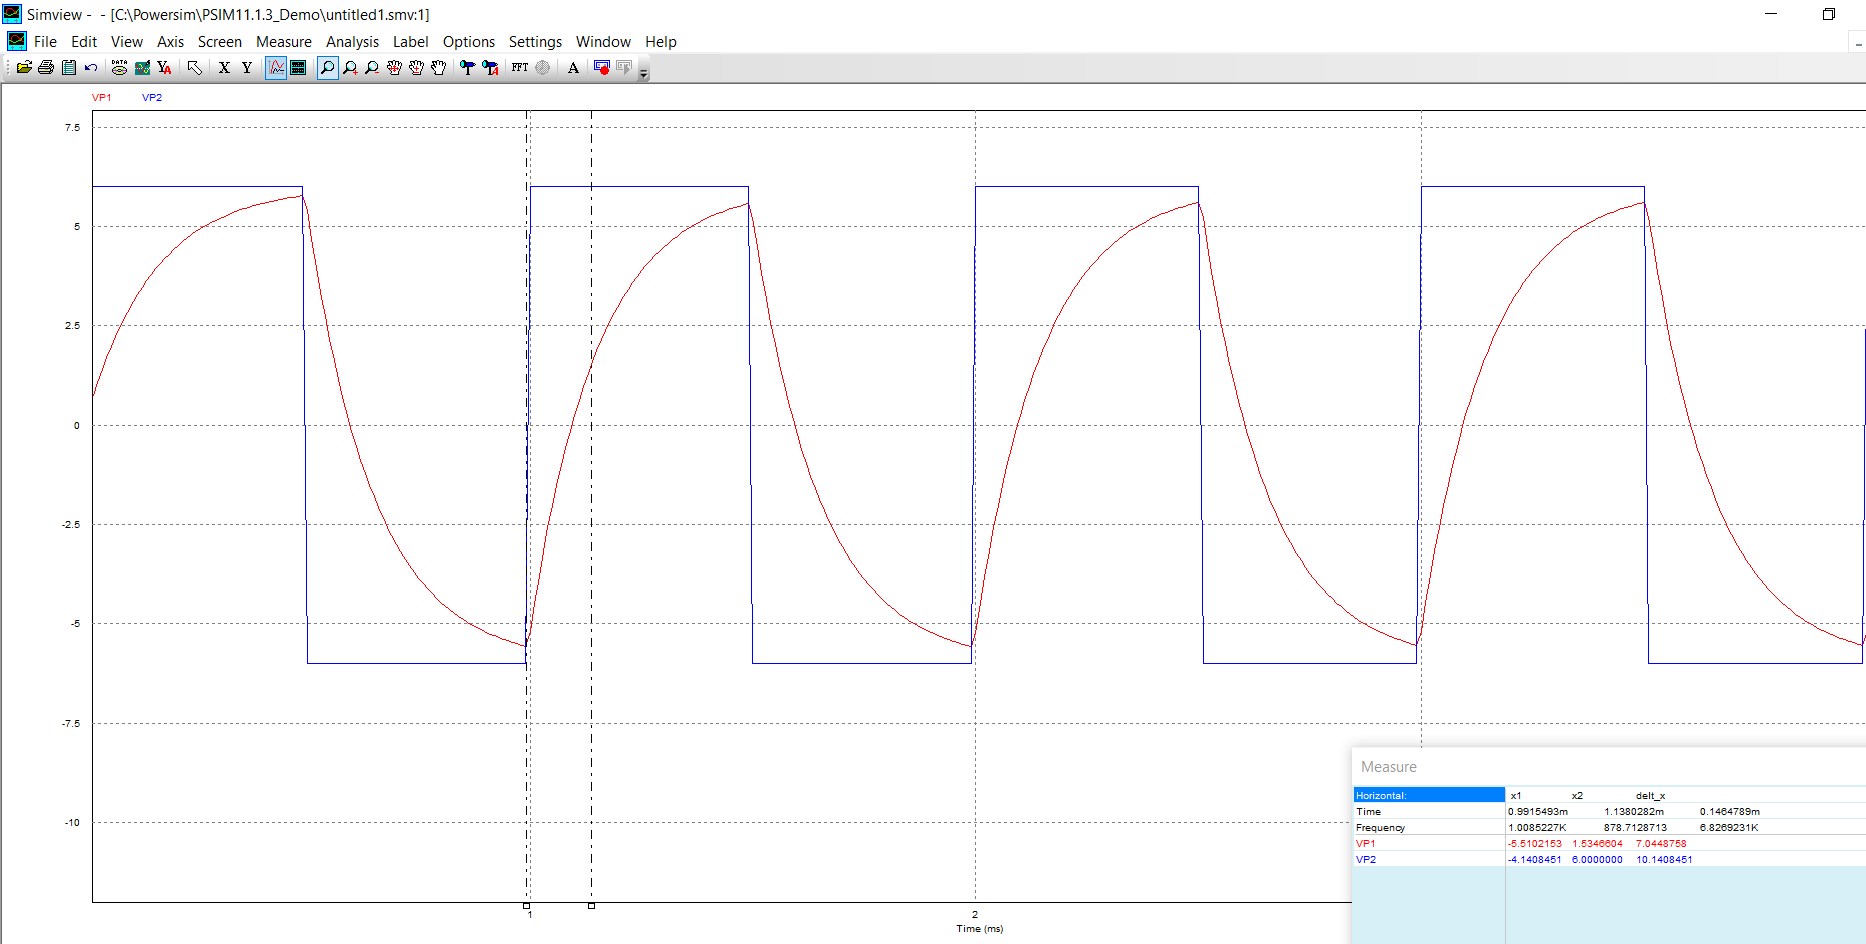
\includegraphics[width = 0.9\textwidth]{Relatorio1_PSIM_Tau.png}
    \caption{Simulação no PSIM\cite{psim}}
    \end{minipage}\hfill
\end{figure}

Para o capacitor carregar 63\% do valor, no micro-cap temos um tempo de 150.876us e no PSIM de aproximadamente 146us. Ambos os simuladores chegaram em resultados parecidos com o esperado, entretanto, pelo fato do Micro-cap ser mais robusto, e não lidar apenas com circuitos ideais, chegou a um resultado mais parecido ao que era esperado.
    
\clearpage
    Para o circuito b), na parte teórica temos o seguinte comportamento:
    
 \begin{figure}[!htb]
    \centering
    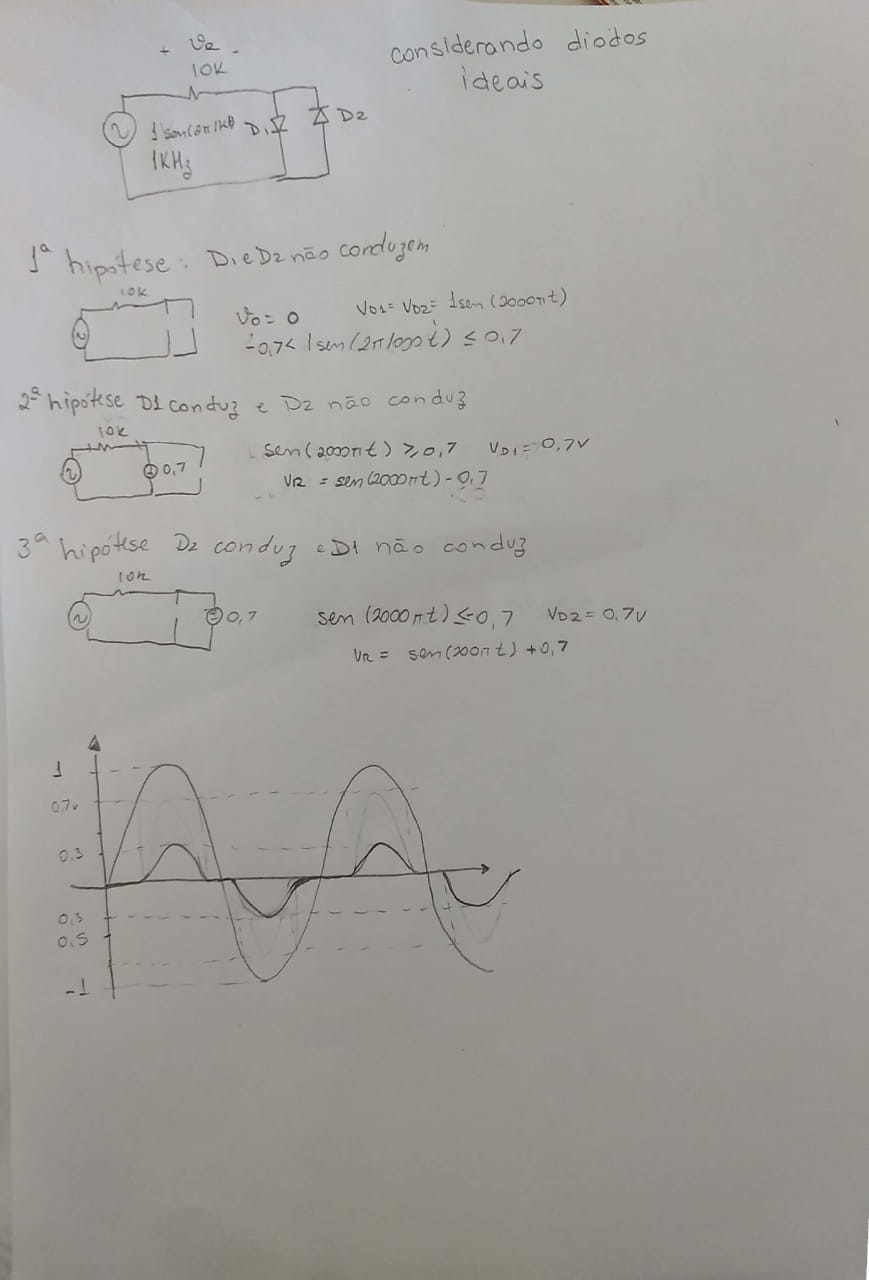
\includegraphics[width=8cm,height=6cm]{Relatorio1_teo_diodo.png}
    \caption{Análise teórica}
\end{figure}
    
    Onde podemos ver que a ddp medida no resistor está em zero até a fonte chegar em 0.7V podendo ser negativo ou positivo e depois disso ela fica a 0.7V a menos que a fonte senoidal. Esse comportamento acontece devido aos diodos em paralelo. Nas simulações, temos:
    
\begin{figure}[!htb]
    \begin{minipage}{0.5\textwidth}
    \centering
    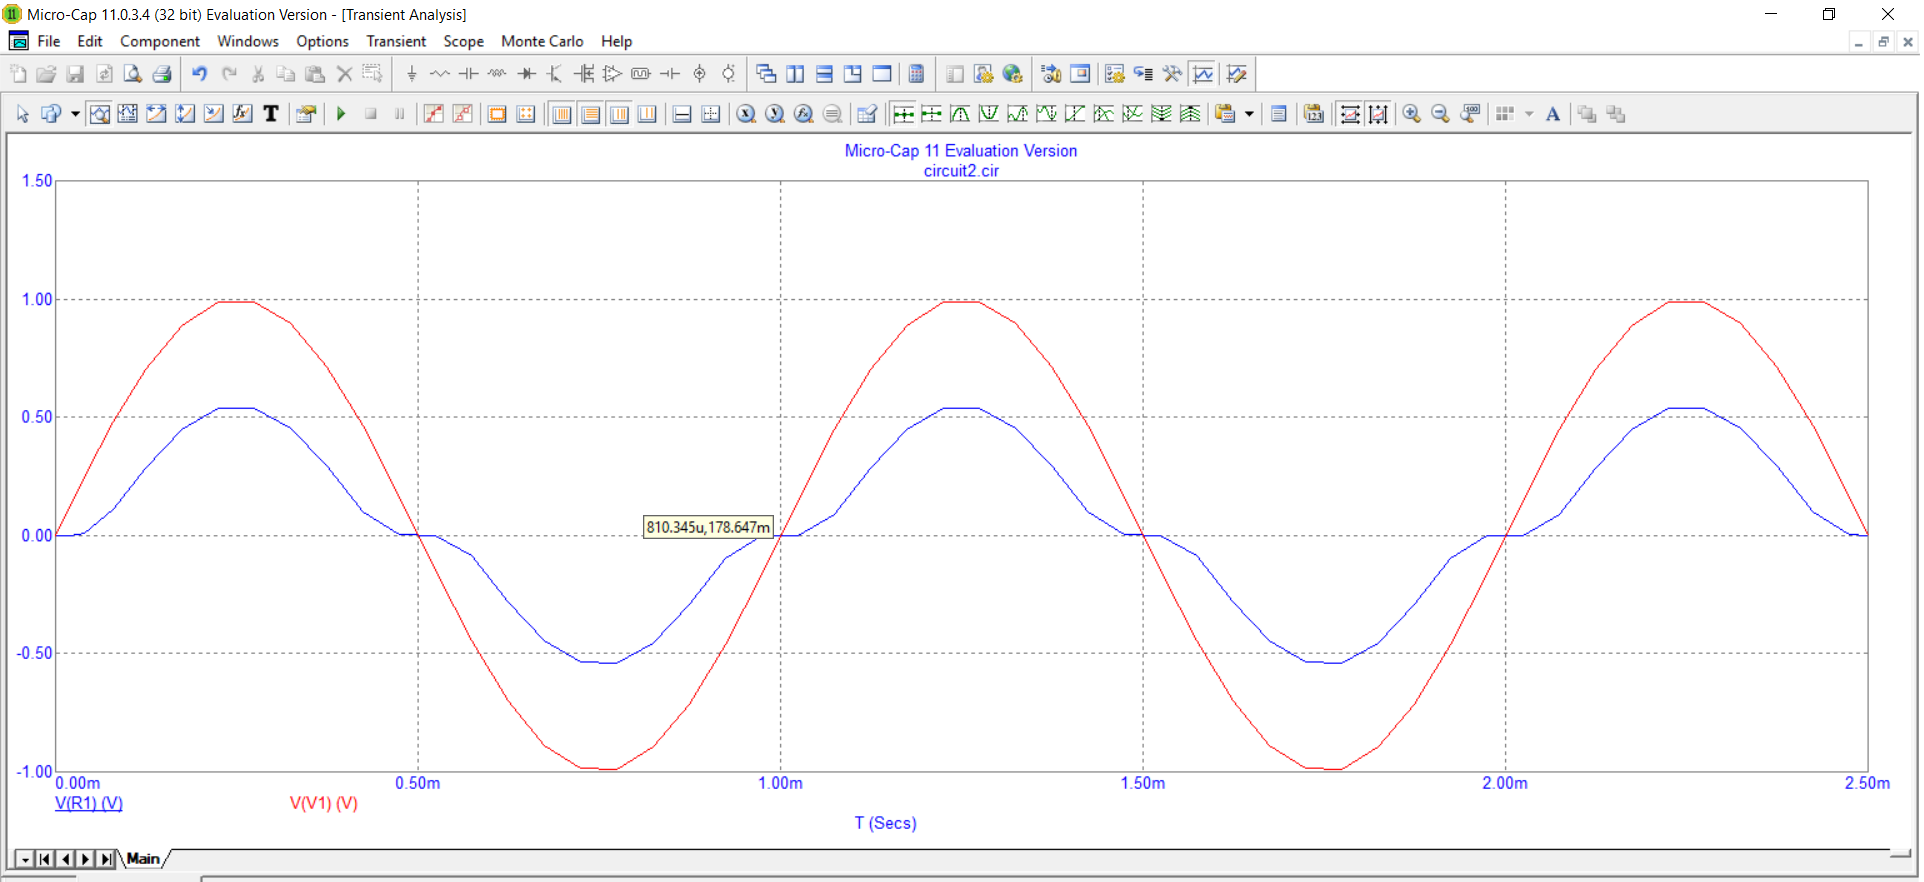
\includegraphics[width = 0.9\textwidth]{Relatorio1_microcap_Diodo.png}
    \caption{Simulação no Micro-cap\cite{microcap}}
    \end{minipage}\hfill
    \begin{minipage}{0.5\textwidth}
    \centering
    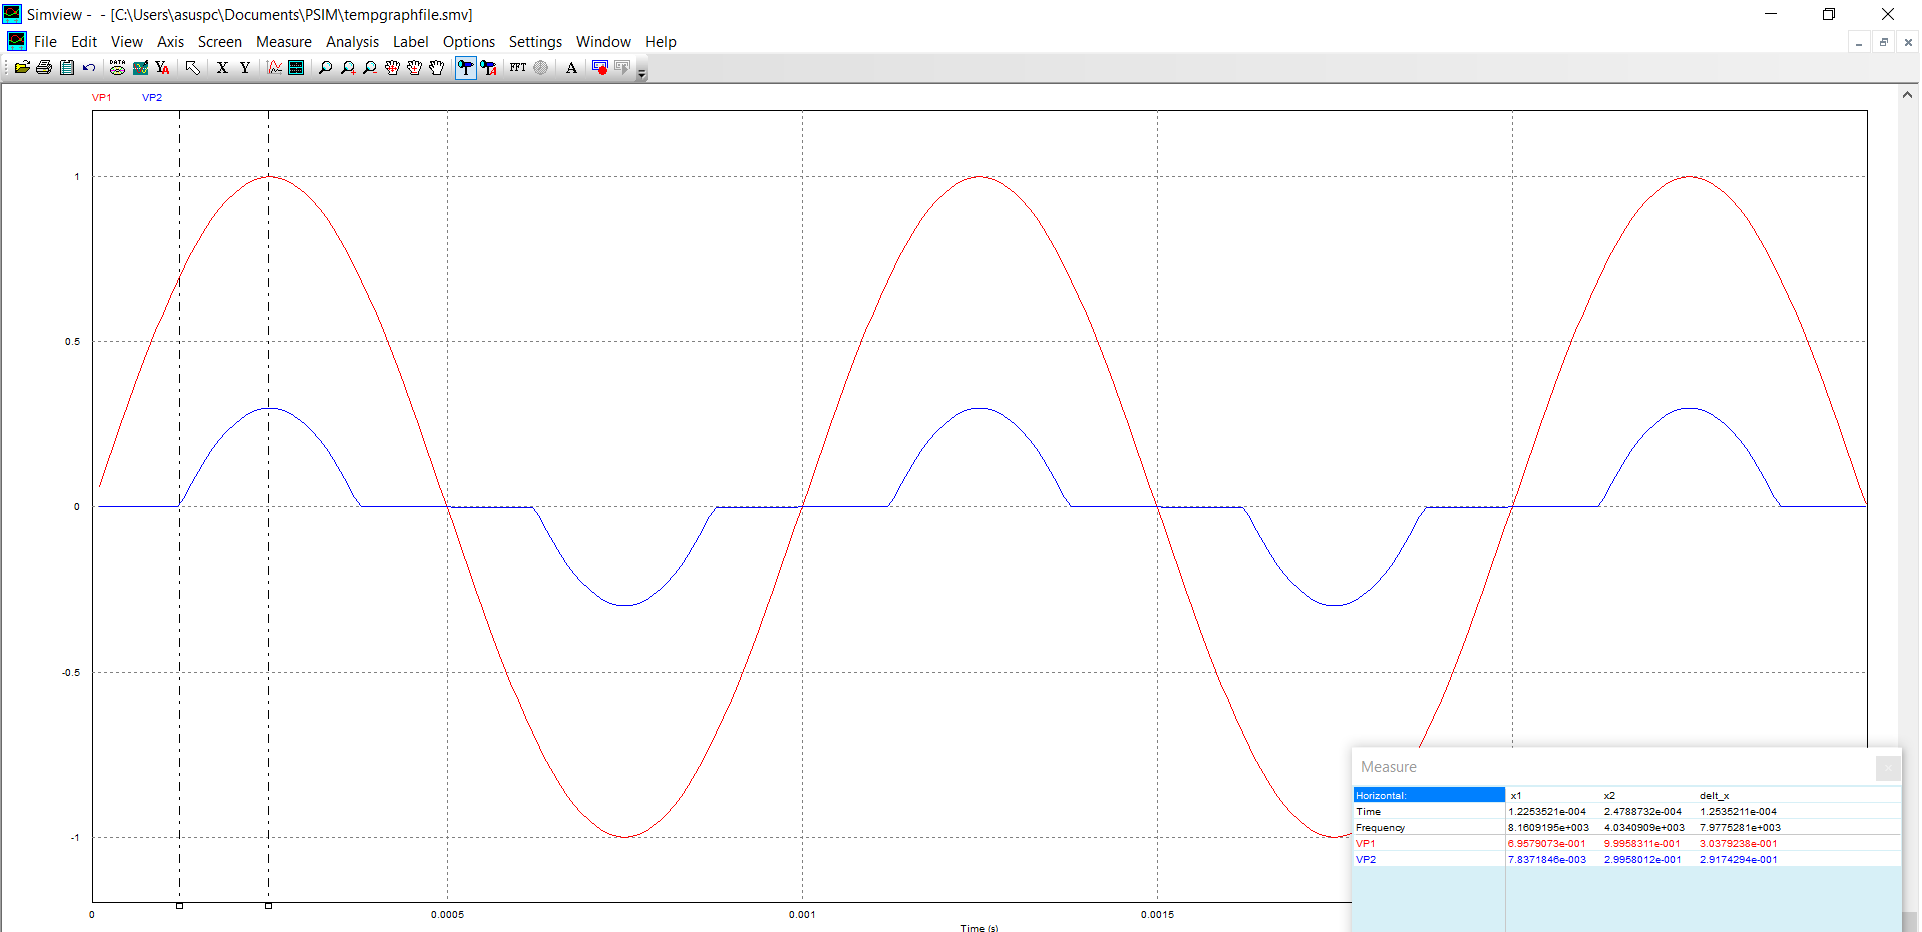
\includegraphics[width = 0.9\textwidth]{Relatorio1_PSIM_Diodo.png}
    \caption{Simulação no PSIM\cite{psim}}
    \end{minipage}\hfill
\end{figure}

  Podemos notar que no PSIM, o resultado ficou muito mais parecido do teórico do que o do Micro-cap. Esse fato ocorre devido ao tipo de diodo utilizado, e o modelo usado pra calcular a forma de onda do mesmo. Na teoria foi utilizado um diodo com 0.7 de \textit{forward voltage} e no PSIM também. Assumimos um comportamento ideal do diodo, logo a resistência interna é zero. Entretanto, no modelo usado no PSIM a resistência interna é de 100m$\Omega$, e o modelo do Micro-cap é o modelo 1N4148.
  
%-----------------------------------------------
%   Projeto de uma Placa de Circuito Impresso 
%
%---------------------------------
\chapter{Projeto de uma Placa de Circuito Impresso }\label{cap_pcb}

Para o projeto da PCI, foi utilizado o software KiCAd\cite{kicad}. Nos era proposto a criação de um circuito RLC, onde o capacitor e o indutor era diferente para cada grupo. Para essa etapa, cada integrante do grupo recebeu dois valores $M$ e $N$, dados pelo professor,fazendo a média dos valores e arredondando para cima, temos novos $M$ e $N$. Esses novos valores que foram utilizados para o dimensionamento do indutor e o tipo de capacitor. No nosso caso, o indutor deveria ter uma altura de 20mm, largura de 50mm e profundidade e 20mm, e nosso capacitor é cerâmico.

\begin{figure}[!htb]
    \begin{minipage}{0.5\textwidth}
    \centering
    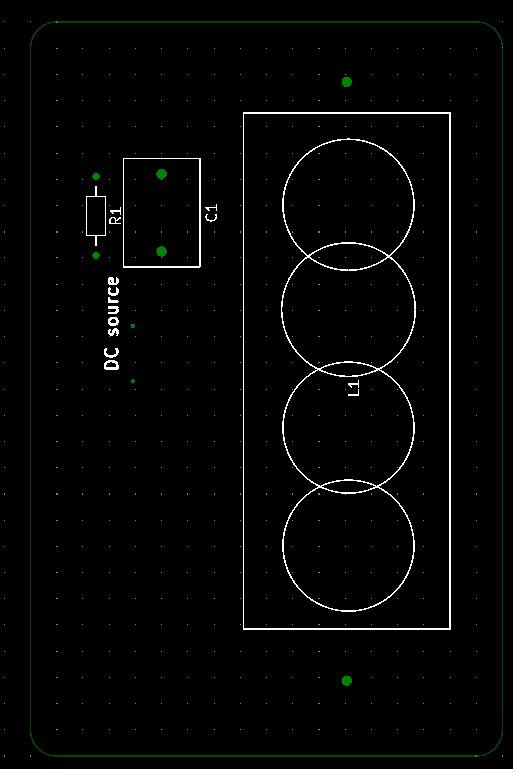
\includegraphics[height = 6cm,width = 0.75\textwidth]{PCB_1.png}
    \caption{Top layer}
    \end{minipage}\hfill
    \begin{minipage}{0.5\textwidth}
    \centering
    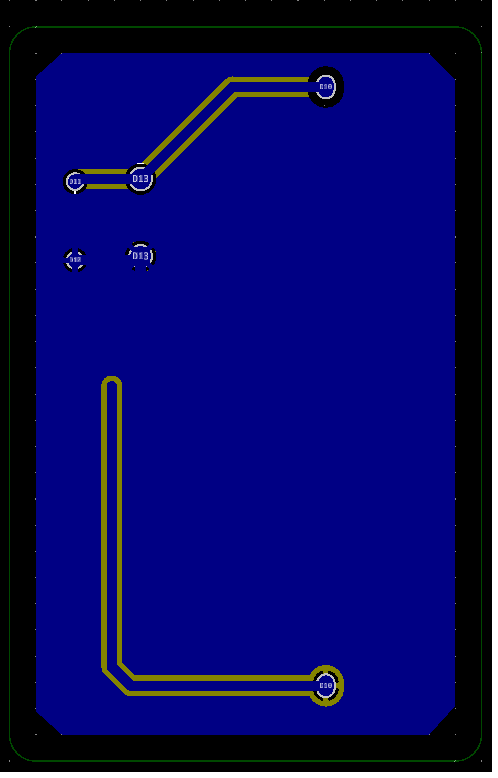
\includegraphics[height = 6cm,width = 0.75\textwidth]{PCB_2.png}
    \caption{Bottom layer}
    \end{minipage}\hfill
\end{figure}

\begin{figure}[!htb]
    \begin{minipage}{0.5\textwidth}
    \centering
    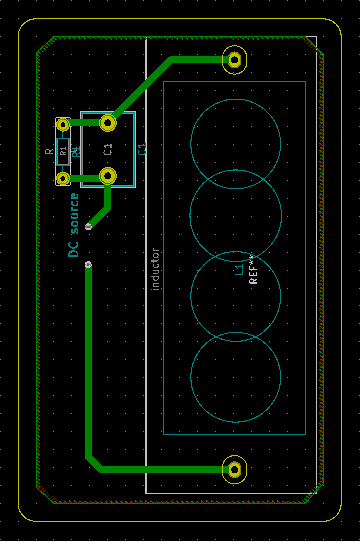
\includegraphics[height = 6cm,width = 0.75\textwidth]{PCB_3.png}
    \caption{Layout}
    \end{minipage}\hfill
    \begin{minipage}{0.5\textwidth}
    \centering
    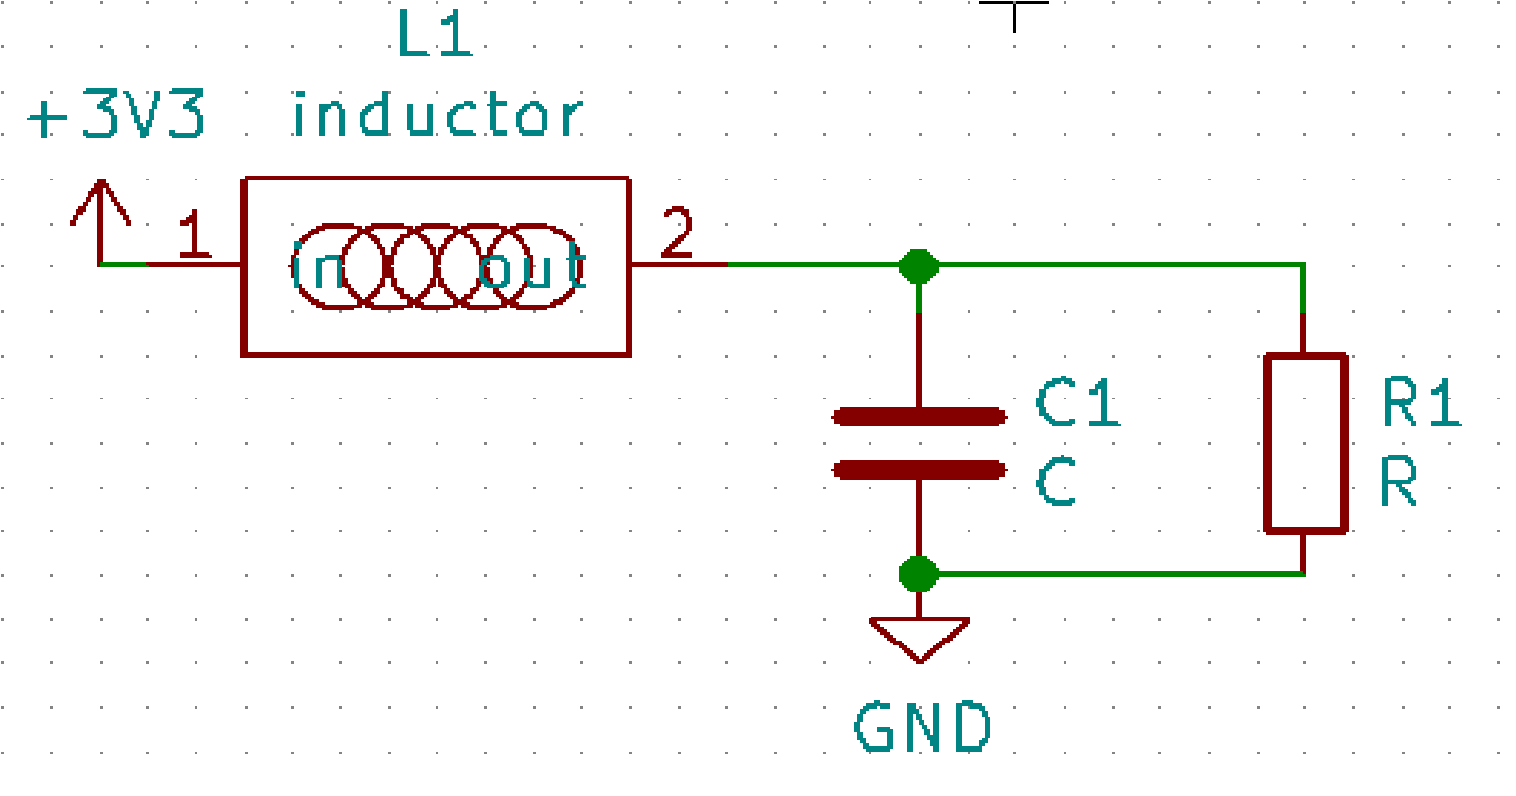
\includegraphics[height = 6cm,width = 0.75\textwidth]{PCB_4.png}
    \caption{Esquemático}
    \end{minipage}\hfill
\end{figure}

\clearpage
Na bottom layer, vemos que não temos uma rota para o ground, isso ocorre porque ela é uma zona preenchida \textit{gnd} assim, só é necessário o ponto de soldagem no capacitor e no resistor para eles estarem conectados ao ground.

%-
%	Conclusão
%
%

% ---

% ----------------------------------------------------------
% ELEMENTOS PÓS-TEXTUAIS
% ----------------------------------------------------------
\postextual

% ----------------------------------------------------------
% Referências bibliográficas
% ----------------------------------------------------------

\bibliography{abntex2-modelo-references}


\end{document}
